\section{Database Implementation}
For implementation, we are using MySQL (8.0).

\subsection{Create Tables}
\begin{minted}{sql}
create table User (
    uemail varchar(50) not null primary key,
    uname varchar(50) null,
    nickname varchar(50) null,
    password varchar(50) null
);

create table Workspace (
    wid int auto_increment primary key,
    wname varchar(50) null,
    wdesc varchar(200) null
);

create table Channel (
    wid int not null,
    cname varchar(50) not null,
    ctype varchar(50) null,
    ctime datetime null,
    primary key (wid, cname),
    foreign key (wid) references Workspace (wid)
);

create table Message (
    wid int not null,
    cname varchar(50) not null,
    uemail varchar(50) not null,
    mtime datetime not null,
    mcontent varchar(300) null,
    primary key (wid, cname, uemail, mtime),
    foreign key (wid, cname) references Channel (wid, cname),
    foreign key (uemail) references User (uemail)
);

create table cInvitation (
	semail varchar(50) not null,
	remail varchar(50) not null,
	wid int not null,
	cname varchar(50) not null,
	citime datetime not null,
	primary key (semail, remail, wid, cname, citime),
    foreign key (semail) references User (uemail),
    foreign key (remail) references User (uemail),
    foreign key (wid, cname) references Channel (wid, cname)
);

create table cMember (
    uemail varchar(50) not null,
    wid int not null,
    cname varchar(50) not null,
    primary key (uemail, wid, cname),
    foreign key (uemail) references User (uemail),
    foreign key (wid, cname) references Channel (wid, cname)
);

create table wInvitation (
    semail varchar(50) not null,
    remail varchar(50) not null,
    wid int not null,
    witime datetime not null,
    primary key (semail, remail, wid, witime),
    foreign key (semail) references User (uemail),
    foreign key (remail) references User (uemail),
    foreign key (wid) references Workspace (wid)
);

create table wMember (
    uemail varchar(50) not null,
    wid int not null,
    wmtype varchar(50) null,
    primary key (uemail, wid),
    foreign key (uemail) references User (uemail),
    foreign key (wid) references Workspace (wid)
);
\end{minted}


\subsection{Insert Testing Data}
For testing purpose, we generated some sampled data as follows:
\begin{itemize}
    \item First, we generated 9 users, 6 workspaces and 7 channels with different types and corresponding workspace.
    \item Then we insert the messages and the relationship between different entities so that we ensure at least some result will show up for each query.
\end{itemize}

\begin{figure}[ht!]
    \centering
    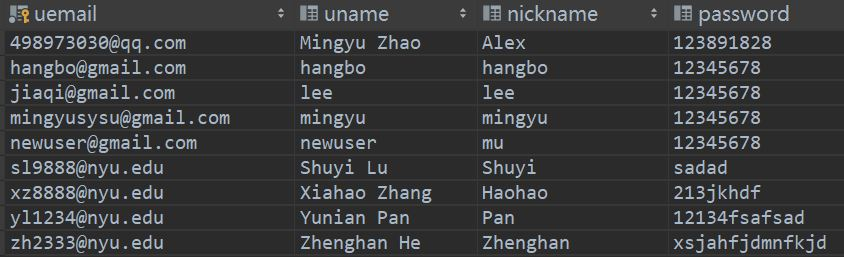
\includegraphics[width=0.9\textwidth]{img/User.JPG}
    \caption{Sampled Data for the \textbf{User} Relation}
\end{figure}

\FloatBarrier

\begin{figure}[ht!]
    \centering
    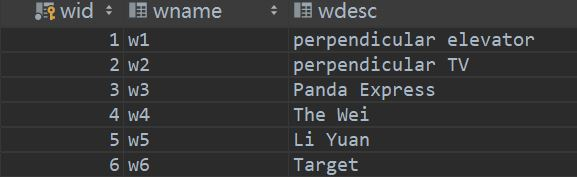
\includegraphics[width=0.75\textwidth]{img/Workspace.JPG}
    \caption{Sampled Data for the \textbf{Workspace} Relation}
\end{figure}

\FloatBarrier

\begin{figure}[ht!]
    \centering
    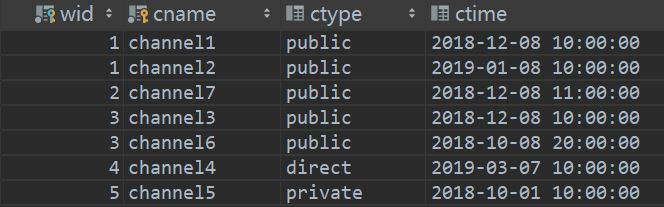
\includegraphics[width=0.75\textwidth]{img/channel.JPG}
    \caption{Sampled Data for the \textbf{Channel} Relation}
\end{figure}

\FloatBarrier

\begin{figure}[ht!]
    \centering
    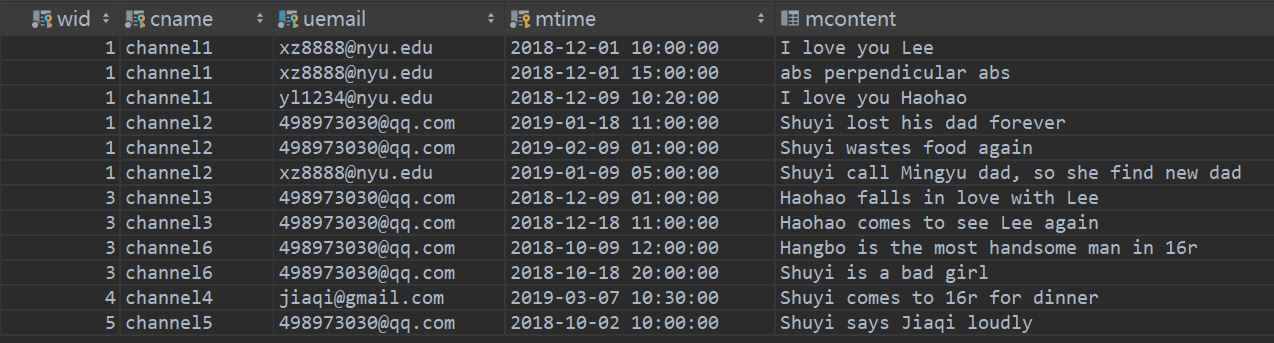
\includegraphics[width=1.0\textwidth]{img/Message.JPG}
    \caption{Sampled Data for the \textbf{Message} Relation}
\end{figure}

\FloatBarrier

\begin{figure}[ht!]
    \centering
    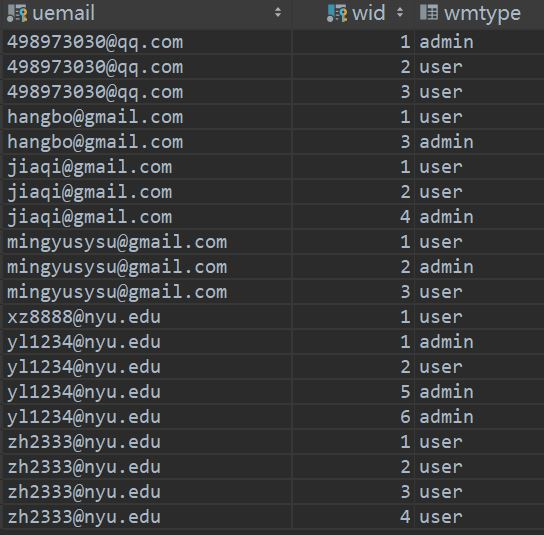
\includegraphics[width=0.95\textwidth]{img/wMember.JPG}
    \caption{Sampled Data for the \textbf{wMember} Relation}
\end{figure}

\FloatBarrier

\begin{figure}[ht!]
    \centering
    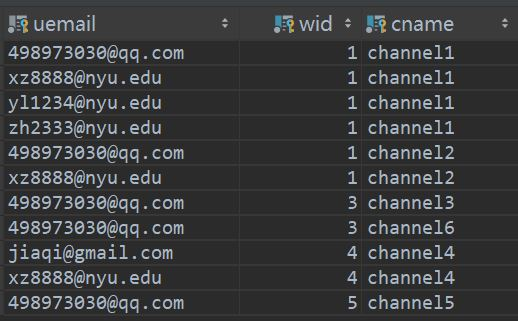
\includegraphics[width=0.8\textwidth]{img/cMember.JPG}
    \caption{Sampled Data for the \textbf{cMember} Relation}
\end{figure}

\FloatBarrier

\begin{figure}[ht!]
    \centering
    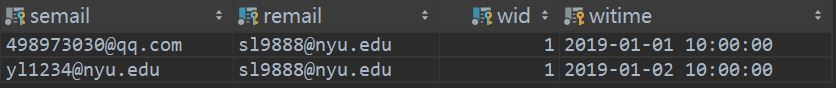
\includegraphics[width=1.0\textwidth]{img/wInvitation.JPG}
    \caption{Sampled Data for the \textbf{wInvitation} Relation}
\end{figure}

\FloatBarrier

\begin{figure}[ht!]
    \centering
    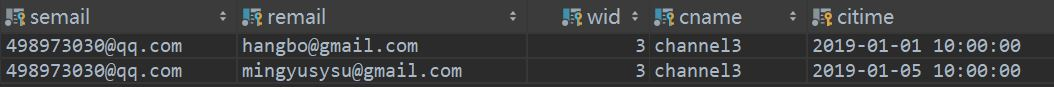
\includegraphics[width=1.0\textwidth]{img/cInvitation.JPG}
    \caption{Sampled Data for the \textbf{cInvitation} Relation}
\end{figure}

\FloatBarrier

\newpage

\subsection{Sample Queries}

\subsubsection{Query 1: Create a new user account, with email, name, nickname, and password.}
SQL Query:
\begin{minted}{sql}
    insert into User
    value ('newuser@gmail.com', 'newuser', 'nu', '12345678');
\end{minted}

\subsubsection{Query 2: Create a new public channel inside a workspace by a particular user.}
SQL Query:
\begin{minted}{sql}
    insert into Channel
    value (2, 'channel7', 'public', '2018-12-08 11:00:00');
\end{minted}

\subsubsection{Query 3: For each workspace, list all current administrators.}
SQL Query:
\begin{minted}{sql}
    select uemail, wid
    from Workspace natural join wMember
    where wmtype = 'admin'
    group by uemail, wid;
\end{minted}

Query Result:
\begin{figure}[ht!]
    \centering
    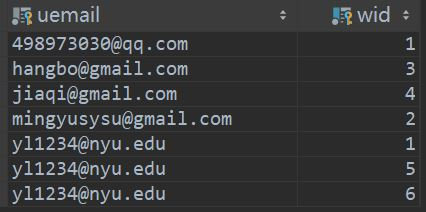
\includegraphics[width=0.4\textwidth]{img/sql3.JPG}
\end{figure}

\subsubsection{Query 4: For each public channel in a given workspace, list the number of users that were invited to join the channel more than
5 days ago and that have not yet joined.}
SQL Query:
\begin{minted}{sql}
    select wid, cname, count(remail) as allnotin
from cInvitation natural join Channel
where timestampdiff(Day, (date_format(ctime,'%Y%m%d')),date_format(now(),'%Y%m%d')) > 5 and wid = 3
  and Channel.ctype = 'public'
      and remail not in (
        select uemail
        from cMember
        where wid = 3 and cInvitation.cname = cMember.cname
    )
group by wid, cname;
\end{minted}

Query Result:
\begin{figure}[ht!]
    \centering
    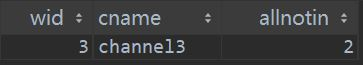
\includegraphics[width=0.4\textwidth]{img/sql4.JPG}
\end{figure}

\subsubsection{Query 5: For a particular channel, list all messages in chronological order.}
SQL Query:
\begin{minted}{sql}
    select mcontent
    from Channel natural join Message
    where cname = 'channel1'
    order by mtime;
\end{minted}

Query Result:
\begin{figure}[ht!]
    \centering
    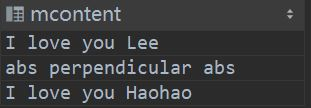
\includegraphics[width=0.35\textwidth]{img/sql5.JPG}
\end{figure}

\subsubsection{Query 6: For a particular user, list all messages they have posted in any channel.}
SQL Query:
\begin{minted}{sql}
    select mcontent
    from Message
    where uemail = '498973030@qq.com';
\end{minted}

Query Result:
\begin{figure}[ht!]
    \centering
    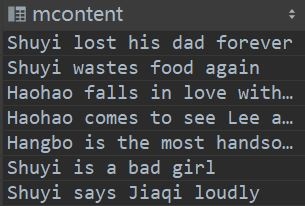
\includegraphics[width=0.4\textwidth]{img/sql6.JPG}
\end{figure}

\subsubsection{Query 7: For a particular, list all messages that are accessible to this user and that contain the keyword “perpendicular” in the
body of the message.}
SQL Query:
\begin{minted}{sql}
    select mcontent
    from Message natural join cMember natural join wMember
    where uemail = 'xz8888@nyu.edu' and mcontent like '%perpendicular%';
\end{minted}

Query Result:
\begin{figure}[ht!]
    \centering
    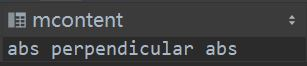
\includegraphics[width=0.4\textwidth]{img/sql7.JPG}
\end{figure}
